The Linear Congruential class of RNGs, or LCG for short, is a very old and relatively simple random number generator. They are based on the formula for a line, modulo another number. The following recurrence relation defines the LCG.
\begin{equation} \label{eq:lcg}
    X_{n+1} = (aX_n + c) \mod m
\end{equation}
Where the parameters are chosen with the following restraints:
\begin{align*}
    m,   \qquad & 0 < m \\
    a,   \qquad & 0 < a < m \\
    c,   \qquad & 0 \leq c < m \\
    X_0, \qquad & 0 \leq X_0 < m
\end{align*}
If $c = 0$, this particular class of of RNG is called a Lehmer, or Park-Miller RNG \cite{Payne:1969:CLP:362848.362860,Park:1988:RNG:63039.63042}.

The period of such generators depends heavily on the chosen parameters. It can be at most $m$, and as a result, $m$ is often chosen to be the largest number which can fit in the number of bits of the output; usually $2^{32}$ or $2^{64}$. Some common parameter sets in use include MINSTD, and glibc. A set of parameters notoriously deemed unfit for use is called RANDU, and is discussed below. Values for these parameters can be found in

\begin{table}[tb]
    \caption{Table of common LCG parameters.}
    \label{tab:lcg_params}
    \begin{center}
        \begin{tabular}{l|ccc}
        \hline
        \hline
        \textbf{Name} & $m$ & $a$ & $c$ \\
        \hline
            MINSTD & $2^{32} - 1$ & 48271 & 0 \\
            glibc & $2^{31}$ & 1103515245 & 12345 \\
            RANDU & $2^{31}$ & 65539 & 0 \\
        \hline
        \hline
        \end{tabular}
    \end{center}
\end{table}

\subsubsection{Strengths}
LCG generators are tiny. They store a single word of state, are easy to seed, and with proper parameter choosing can be quite effective RNGs. However, some of the flaws greatly outweigh the lightweight and speed benefits of LCGs for all but the most basic of platforms, discussed next.

\subsubsection{Weaknesses}

LCGs have a fatal flaw, that is amplified by bad parameter choosing: their outputs fall in easily identifiable planes, as proved by Marsaglia \cite{randomnumbersinplanes}. This is most easily demonstrated by viewing the output of a notoriously bad set of parameters: RANDU. In Figure~\ref{fig:randu_fig}, the output of RANDU is treated as $(x,y,z)$ pairs as it is generated, then these points are plotted. It is obvious that all of the output falls in the same set of planes, and is not even an approximation of a truly random number generator. Better parameter choices alleviate this phenomenon by adding the number of planes that would come up in a test like this, and making them closer together, but the basic problem is unavoidable.

Another issue is the period length; at most the period length is $m$, which cannot be easily increased without increasing the number of bits in the word being operated on, which is not practical on modern architectures. In fact, experts recommend not even considering generators with periods $<2^{50}$ for anything but the most trivial uses \cite{L'Ecuyer:1992:TRN:167293.167354}.

\begin{figure}[tb]
    \begin{center}
        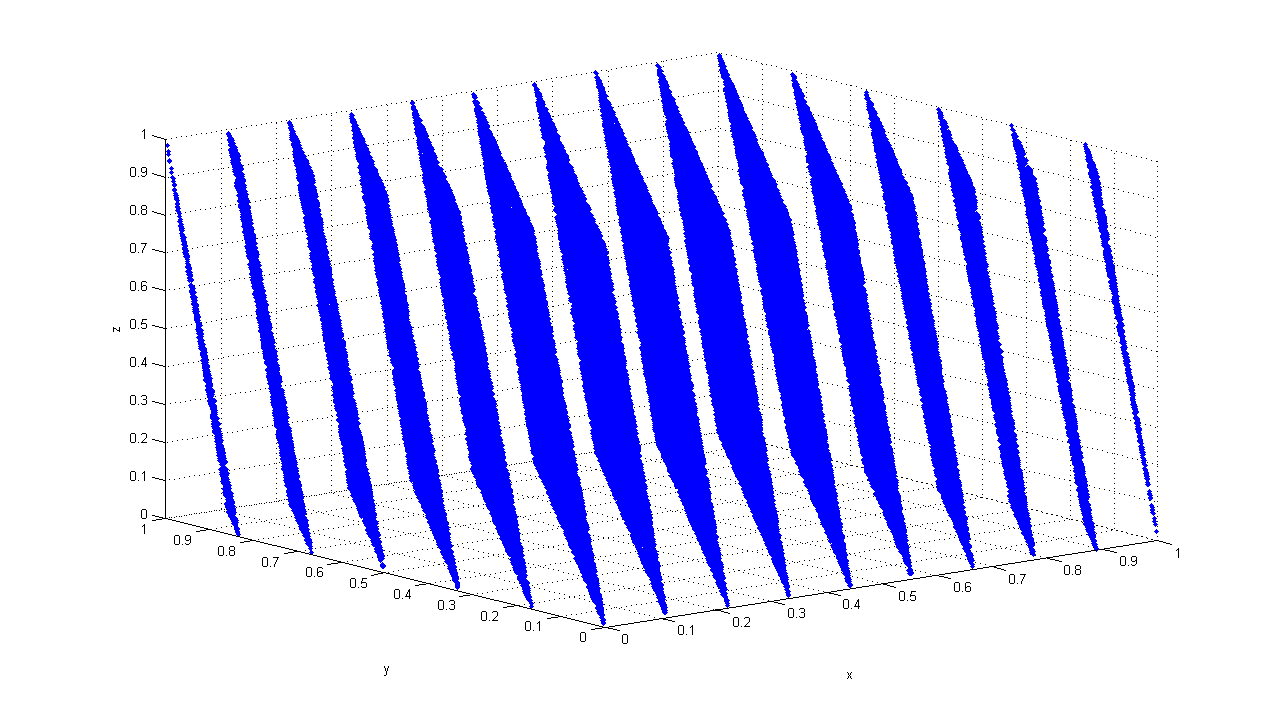
\includegraphics[width=\linewidth]{figures/randu.png}
    \end{center}
    \caption{The problem with LCGs demonstrated by RANDU; a MATLAB plot of consecutive outputs from RANDU used as $(x,y,z)$ points and plotted \cite{randu_fig}.}
    \label{fig:randu_fig}
\end{figure}

Despite these flaws, these extremely small and fast RNGs may still be suited to small embedded architectures and applications where speed is significantly more important than quality.
